\section{\nn{} Runtime Energy Adaptation} \label{sec:method2}

\nn{} runtime energy adaptation utilises the presented runtime energy profiling to dynamically adapts the voltage threshold to the latest energy consumption of a task. 
The adaptation method assumes the system is able to monitor the supply voltage and signal the MCU to wake up or sleep when a high or low threshold is hit, and the threshold is configurable by the MCU at runtime. 
In practice, this voltage monitoring ability is widely adopted by IPSs in the forms of a voltage comparator~\cite{kang2018homerun, balsamo2016hibernus++}, an energy management unit~\cite{gomez2016dynamic, maeng2019supporting}, or a periodic ADC polling~\cite{sliper2019efficient}. 

% Goal
The fundamental goal of the runtime energy adaptation is to allocate a barely sufficient energy budget for each task. 
Utilising the presented runtime energy profiling method, \nn{} is able to obtain the latest $\Delta \nmm{V}{task}$ of a task and update its threshold accordingly. 
The voltage threshold \nm{V}{th} of a barely sufficient energy budget is defined as:
\begin{equation}
    \nmm{V}{th} = \Delta \nmm{V}{task} + \nmm{V}{end}
    \label{eq:vth_definition}
\end{equation}
where \nm{V}{end} is the target end voltage below which the whole or part of system's hardware cannot function correctly. 
\nm{V}{end} can be higher than the MCU shutdown voltage, e.g. a peripheral that has a higher operating voltage. 
Besides allocating the lowest \nm{V}{th}, an ideal adaptation scheme is also expected to have low overheads, run energy profiling only when necessary, and react to energy variations immediately.

Based on the above aims, we design \nn{}'s runtime adaptation scheme. 
It consists of a basic adaptation routine for a fixed workload and an optional linear adaptation method for workloads that has a linearly-scaled $\Delta \nmm{V}{task}$ with dynamic parameters.
\nn{}'s runtime energy adaptation is decoupled with the energy profiling method. 
The adaptation scheme allows the energy profiling method to be integrated in the routine but only requires an interface which allows it to trigger an instance of profiling and return a profiling result.

% Enable voltage threshold adaptation against runtime variation of energy consumption due to unforeseeable operating conditions, and also enable linear adaptation to function knobs that are known to the system. 

\subsection{Adaptation Routine}

\begin{figure}
    \centering
    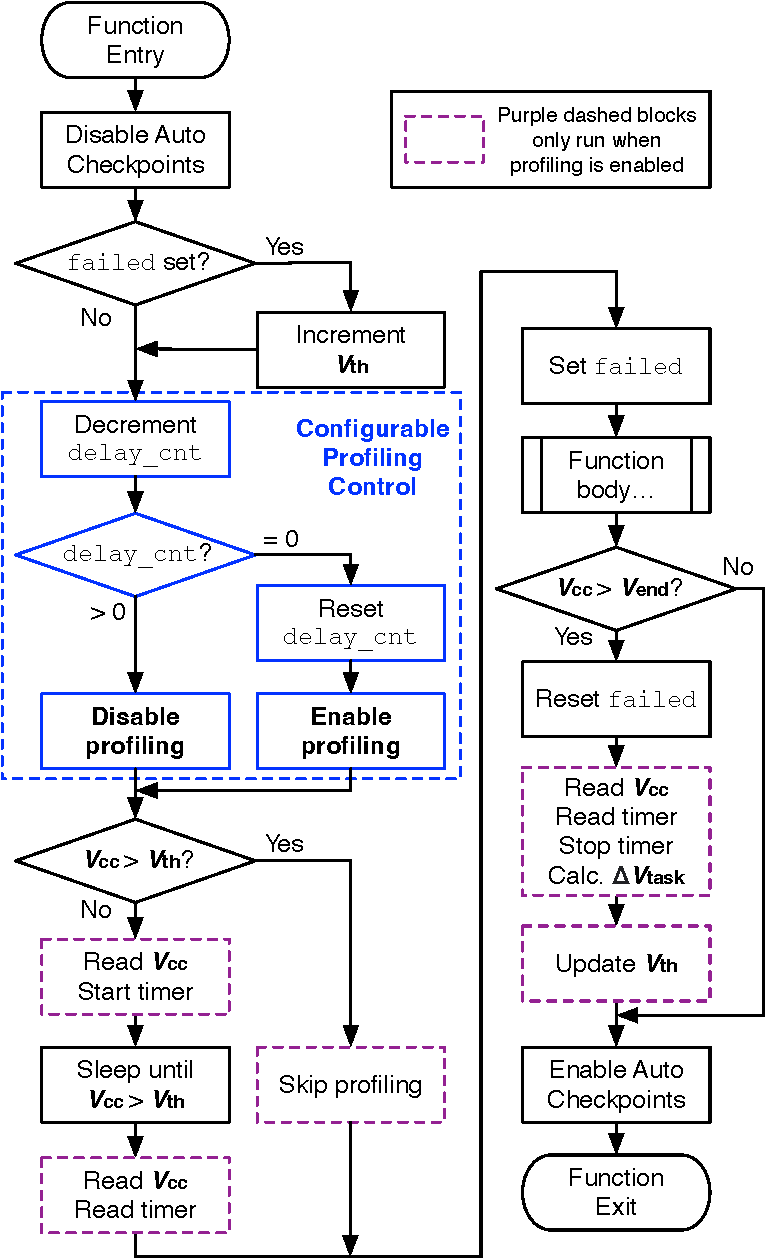
\includegraphics[width=0.8\columnwidth]{ch5_optic/figures/flowchart.pdf}
    \caption{Flowchart of \nn{}'s runtime energy adaptation routine. The blue blocks represent a configurable control logic to decide when to perform energy profiling. The dashed purple blocks are only run when the profiling is enabled, and represent \nn{}'s energy profiling with the last block updating \nm{V}{th} with the new $\Delta \nmm{V}{task}$. }
    \label{fig:opta_flowchart}
\end{figure}

A flowchart of \nn{}'s adaptation routine is shown in \fref{fig:opta_flowchart}.
The routine operates at the entry and the exit of a task.
Checkpoints are disabled during the atomic task, so the program rolls back to a point before the task entry if a power interruption happens between the entry and the exit.
The system executes the task body when \nm{V}{cc} is above \nm{V}{th}. If \nm{V}{cc} is below \nm{V}{th}, the system sleeps and waits until \nm{V}{th} is reached.

A non-volatile flag, "failed", is assigned for each task in order to monitor whether \nm{V}{end} is met with the current \nm{V}{th}.
The "failed" flag is set when a power interruption happens in the task body or when \nm{V}{cc} falls below \nm{V}{end} after the task body finishes. 
At the entry of a task, \nn{} checks whether "failed" is set, i.e. whether \nm{V}{th} fails to meet \nm{V}{end} last time, and increment \nm{V}{th} if it is set. 
The increment amount can be dependent on volatility of energy consumption and the resolution of the adopted voltage monitor. 
In practice (\sref{sec:implementation}), we found that incrementing one unit step of the voltage monitor, which corresponds to about \SI{30}{\milli\volt} in our implementation, suffices both stability and reactivity. 

Following the failure check, the routine has a control of when to trigger energy profiling (blue blocks in \fref{fig:opta_flowchart}), such that energy profiling is not performed every time that the task is run so as to save the energy and time overheads on unnecessary profiling. 
The control logic can be configured as per the requirements of users or applications. 
We have exemplified this with a delay counter, where the energy profiling is enabled every a number of completions. 
Alternatively, persistent timekeepers~\cite{winkel2020reliable, deep2020harc, hester2016persistent} can also be used to trigger energy profiling once a period of real time passes.

If energy profiling is enabled, the dashed purple blocks in \fref{fig:opta_flowchart} are performed in the routine. 
The particular operations involved can be dependent on the profiling method, while we have illustrated this in the flowchart with \nn{}'s profiling method. 
As explained, \nn{}' energy profiling operates at three points when the charge cycle starts, when the charge cycle ends and the discharge cycle starts, and when the discharge cycle ends. 
\nm{V}{th} is then updated after a new $\Delta\nmm{V}{task}$ is profiled following \eref{eq:vth_definition}. 
If a charge cycle is not needed, i.e. the energy stored is already sufficient for the task, the profiling is skipped and performed next time as this contradicts the design of \nn{}'s profiling method.

% optional linear adaptation
% optional multiple configurations (can be similar to multiple atom_func_state)
\subsection{Linear Adaptation}

The above threshold adaptation is design for workloads that have a fixed amount of computational work and a determined configuration, the $\Delta\nmm{V}{task}$ variation of which can change slowly with non-computational factors, e.g. capacitor ageing or temperature variations.
For workloads that have runtime changeable parameters that scale energy consumption significantly, e.g. data sizes and peripheral configurations, the above adaptation can cost a number of failures before adapting to the new threshold. 
While dynamic configurations can be solved with multiple thresholds that switched by the configuration, data sizes can be fine-grained and can introduce a high memory overhead considering the number of thresholds needed. 
Hence, we propose a linear adaptation method as an option for workloads that have linearly-scaled energy consumption with its parameter. 

Thus, a linearly-scaled $\Delta\nmm{V}{task}$ can be represented as:
\begin{equation}
    \Delta\nmm{V}{task} = \nmm{\theta}{1} x + \nmm{\theta}{0}
\end{equation}
where \N{x}{} is the parameter that is supposed to scale $\Delta\nmm{V}{task}$. \nm{\theta}{1} and \nm{\theta}{0} are the slope and y-intercept of the linear relationship between $\Delta\nmm{V}{task}$ and \nm{x}{}. Hence, \nm{V}{th} for the task should be set as:
\begin{equation}
    \nmm{V}{th} = \nmm{\theta}{1} x + \nmm{\theta}{0} + \nmm{V}{end}
\end{equation}

A straightforward solution to obtain \nm{\theta}{1} and \nm{\theta}{0} can be taking a series of profiling results and calculating the regression function.
Though viable, this can introduce relatively high overheads on sampling and calculation.

To lower the overheads, we adopt an efficient method where energy profiling is performed to update \nm{\theta}{1} and \nm{\theta}{0} when \N{x} reaches its minimum or maximum values. 
\nm{\theta}{1} and \nm{\theta}{0} can then be calculated with less computation than linear regression. 
When the task is run with a \N{x} value other than the minimum or maximum, the energy profiling is disabled and \nm{\theta}{0} is incremented when necessary, e.g. a \N{x} value that causes a higher $\Delta\nmm{V}{task}$ than what the equation predicts. 

The routine of the linear adaptation method is then similar to the one shown in \fref{fig:opta_flowchart}, with modifications on the profiling control and the increment and update of \nm{V}{th}, where it controls whether to profile based on \N{x}, increments \nm{\theta}{0}, and updates \nm{\theta}{1} and \nm{\theta}{0} rather than \nm{V}{th}. 


\todo[inline]{Discussion on e.g. adaptation to other non-linear relationship, the ability to fall back differentiates it from a "simply-incrementing-threshold" approach?}

